% !Mode:: "TeX:UTF-8"
% !TEX program  = xelatex

\documentclass{cumcmthesis}
%\documentclass[withoutpreface,bwprint]{cumcmthesis} %去掉封面与编号页

\usepackage[framemethod=TikZ]{mdframed}
\usepackage{lmodern}
\usepackage{pgfplots}                                                 
\pgfplotsset{compat = 1.8}
\pgfplotsset{every axis label/.append style={font=\small}}
\pgfplotsset{every tick label/.append style={font=\small}}  
\setmainfont{Times New Roman}
% 配置代码高亮
\usepackage{listings}
\lstset{
	basicstyle          =   \sffamily,          % 基本代码风格
	keywordstyle        =   \bfseries,          % 关键字风格
	commentstyle        =   \rmfamily\itshape,  % 注释的风格,斜体
	stringstyle         =   \ttfamily,  % 字符串风格
	flexiblecolumns,                % 别问为什么,加上这个
	numbers             =   left,   % 行号的位置在左边
	showspaces          =   false,  % 是否显示空格,显示了有点乱,所以不现实了
	numberstyle         =   \zihao{-5}\ttfamily,    % 行号的样式,小五号,tt等宽字体
	showstringspaces    =   false,
	captionpos          =   t,      % 这段代码的名字所呈现的位置,t指的是top上面
	frame               =   lrtb,   % 显示边框
}
\lstdefinestyle{Python}{
	language        =   Python, % 语言选Python
	basicstyle      =   \zihao{-5}\ttfamily,
	numberstyle     =   \zihao{-5}\ttfamily,
	keywordstyle    =   \color{blue},
	keywordstyle    =   [2] \color{teal},
	stringstyle     =   \color{magenta},
	commentstyle    =   \color{red}\ttfamily,
	breaklines      =   true,   % 自动换行,建议不要写太长的行
	columns         =   fixed,  % 如果不加这一句,字间距就不固定,很丑,必须加
	basewidth       =   0.5em,
}



\title{高压油管的压力控制}
\tihao{A}
\baominghao{201901001042}
\schoolname{北京大学}
\membera{谭淞宸}
\memberb{曹宇创}
\memberc{李婧宜}
\supervisor{无}
\yearinput{2019}
\monthinput{09}
\dayinput{13}

\begin{document}

 \maketitle
 \begin{abstract}
高压油管被广泛应用于柴油机等燃油发动机中,燃油经过高压油泵进入高压油管,再由喷口喷出。燃油的周期性进入与喷出直接影响其所匹配燃油机性能的稳定性和工作的可靠性。具体而言,管内压力的波动将导致排气温度不稳定,降低了催化剂的转换效率,使燃油机排放一致性下降。因此,减小管内压力的波动,是当前高压燃油系统亟需解决的技术难题。
\par 对于问题一:
\par 对于问题二:
\par 对于问题三:
\par 最后,









\end{abstract}

%目录  2019 明确不要目录,我觉得这个规定太好了
%\tableofcontents

%\newpage
\section{问题的重述}
\subsection{引言}
燃油进入和喷出高压油管是许多燃油发动机工作的基础,图 1 给出了某高压 燃油系统的工作原理,燃油经过高压油泵从 A 处进入高压油管,再由喷口 B 喷 出。燃油进入和喷出的间歇性工作过程会导致高压油管内压力的变化,使得所喷 出的燃油量出现偏差,从而影响发动机的工作效率。

\begin{figure}[h]
	\centering
	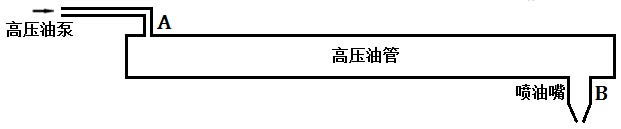
\includegraphics[scale = 1.2]{sketch.jpg}
	\caption{高压油管示意图}
\end{figure}

\subsection{问题的提出}
\subsubsection{问题一}
某型号高压油管的内腔长度为 500mm,内直径为 10mm,供油入口
A 处小孔的直径为 1.4mm,通过单向阀开关控制供油时间的长短,单向阀每打开 一次后就要关闭 10ms。喷油器每秒工作 10 次,每次工作时喷油时间为 2.4ms, 喷油器工作时从喷油嘴 B 处向外喷油的速率如图 2 所示。高压油泵在入口 A 处 提供的压力恒为 160 MPa,高压油管内的初始压力为 100 MPa。如果要将高压油 管内的压力尽可能稳定在 100 MPa 左右,如何设置单向阀每次开启的时长?如 果要将高压油管内的压力从 100 MPa 增加到 150 MPa,且分别经过约 2 s、5 s 和 10 s 的调整过程后稳定在 150 MPa,单向阀开启的时长应如何调整?

\newpage

\section{问题的分析}
\subsection{问题一的分析}
\subsubsection{第一问}
问题一的第一问要求我们通过设置单向阀每次开启的时长,来使得高压油管内的压力稳定在 $1\times10^5~\mathrm{kPa}$。由题目所给信息,在喷油器的一个工作周期($100~\mathrm{ms}$)内,喷油器喷出的油量为 $44~\mathrm{mm^3}$,而油管的容积为 $3.93\times 10^4~\mathrm{mm^3}$,可见油管中的油量变化在 $0.1\%$ 上下,可以近似认为压强不变。

在一个工作周期内,喷油器喷出的流量已知;且在压强不变的近似下,单向阀流入的流速也已知,因而我们可以根据质量守恒定律列出一个工作周期内单向阀应当开启的时间,进行等比例转换后即能得到单向阀每次开启的时间。

在上述讨论过程中,忽略了高压油管内的压强变化,并且忽略了同一时间段内单向阀和喷油器的相互影响,这一影响的大小可以通过对体系进行精确的数值模拟来考察。在数值模拟中,我们采取较小的时间步长(如 $0.01~\mathrm{ms}$),在每一步完成以下计算:

\begin{enumerate}
	\item 检查该时刻单向阀是否处于开启状态;
	\item 如果开启,根据两边压强计算单向阀流入的流量;
	\item 检查该时刻喷油嘴是否处于开启状态;
	\item 如果开启,根据题目所给的流速随时间变化关系计算喷油嘴流出的流量;
	\item 将出入流量乘以相应密度换算为高压油管内燃油的质量变化,进而计算得到更新后的油管内燃油密度;
	\item 将油管内燃油密度的变化通过弹性模量转化为油管内压强的变化;
	\item 将上一步得到的压强继续用于下一步的计算。
\end{enumerate}

通过数值模拟方法,我们可以得到任意时刻油管内的压强,进而计算压强相对于 $10^5~\mathrm{kPa}$ 的偏离幅度大小,进而验证我们通过质量守恒定律选取的开启时间是否是使得系统偏离幅度大小最小的开启时间。



\subsection{问题二的分析}
\subsection{问题三的分析}
\newpage


\section{模型的建立与求解}
\subsection{符号说明}
\begin{table}[!ht]
	\begin{minipage}{\textwidth}
		\begin{minipage}[t]{0.5\textwidth}
			\centering
			\caption{符号说明}
			\begin{tabular}{cc}
			        \toprule
			符号             & 物理量           \\
			\midrule
			$P_1$          & 油泵压力          \\
			$V_1$          & 油泵体积          \\
			$\rho_1$       & 油泵中燃油密度       \\
			$P_2$          & 油管压力          \\
			$P_2^*$        & 目标油管压力        \\
			$d_2$          & 油管直径          \\
			$l_2$          & 油管长度          \\
			$V_2$          & 油管体积          \\
			$\rho_2$       & 油管中燃油密度       \\
			$d_A$          & A 处小孔直径       \\
			$S_A$          & A 处小孔面积       \\
			$Q_A$          & A 处小孔流量       \\ \bottomrule
		\end{tabular}
	\end{minipage}
\begin{minipage}[t]{0.5\textwidth}
\centering
\caption{符号说明}
\begin{tabular}{cc}
\toprule
符号             & 物理量           \\
\midrule
$d_B$          & B 处喷孔直径       \\
$S_B$          & B 处喷孔直径       \\
$Q_B$          & B 处喷油嘴流量      \\
$\tau_0$       & 油管的喷油周期       \\
$\tau_A$       & 喷油周期内 A 的开启时间 \\
$\tau_A^+$     & A 每次的开启时间     \\
$\tau_A^-$     & A 每次的关闭时间     \\
$\tau_A^{\pm}$ & A 一次开启/关闭的总时间 \\
$\theta$       & 凸轮各点极角        \\
$\alpha$       & 凸轮极轴方位角       \\
$h$            & 凸轮最高点高度       \\
$\omega$       & 凸轮角速度         \\
$\gamma$       & 圆锥半角          \\
$z$            & 针阀高度          \\ \bottomrule				
				
				
				
			\end{tabular}
		\end{minipage}
	\end{minipage}
\end{table}
本文中,所有长度均以 $\mathrm{mm}$ 为单位,所有质量均以 $\mathrm{mg}$ 为单位,所有时间均以 $\mathrm{ms}$ 为单位。由于压强的量纲为 $\mathrm{ML^{-1}T^{-2}}$,当使用上述三个基本力学量的单位时,压强的自然单位是 $\mathrm{kPa}$,因此本文中所有压强均以 $\mathrm{kPa}$ 为单位。


\newpage


\subsection{问题一的求解}
\subsubsection{第一小问}
\paragraph{理论计算}
首先假设油管的压力近似保持在 $P_2=P_2^*=1.00\times 10^5~\mathrm{kPa}$,因而油管内燃油 密度 $\rho_2$ 为常数。在喷油器的一个工作周期内,从喷油嘴流出的燃油质量,由流速对时间的积分与密度的乘积给出:

$$
\Delta m=\int_0^{\tau_0}Q_B\rho_2\mathrm dt=37.4~\mathrm{mg}
$$

这些质量应当由从单向阀进入的燃油补充,因此在喷油器一个工作周期内,单向阀平均应该开启的时间应当由损失的质量和补充燃油质量的速度决定:

$$
\begin{aligned}
\tau_A&=\frac{\Delta m}{Q_A\rho_1}\\
&=\frac{\Delta m}{\rho_1CA\sqrt{2(P_1-P_2)/\rho_1}}\\
&=2.76~\mathrm{ms}
\end{aligned}
$$

若我们考虑系统进行较长时间的演化,则在一个周期内单向阀平均开启的时间应该与相同。因此,单向阀开启的时长 $\tau_A^+$ 与它关闭的时长 $\tau_A^-$ 应该满足如下比例式:

$$
\frac{\tau_A^+}{\tau_A^-}=\frac{\tau_A}{\tau_0-\tau_A}
$$

代入已知数据,可以求出 $\tau_A=0.284~\mathrm{ms}$。

\paragraph{数值模拟}

在数值模拟中,我们设定初始条件为 $P_2=1.00\times 10^5~{\mathrm{kPa}}$,且时间零点恰好位于喷油器一个工作周期的开始,但可以位于单向阀一个工作周期中的任意一点,该点处相位为 $t_0$。

系统的演化可以用如下关系表示,其中左箭头「$\leftarrow$」是程序设计中的赋值等号:

$$
\begin{aligned}
Q_A &\leftarrow Q_A(t)\\
m_2 &\leftarrow m_2 + Q_A \times \rho_1 \times dt\\
Q_B &\leftarrow Q_B(t)\\
m_2 &\leftarrow m_2 - Q_B \times \rho_2 \times dt\\
\rho_2 &\leftarrow m_2 / V_2\\
P_2 &\leftarrow P(\rho_2)\\
\end{aligned}
$$

将系统进行 $N$ 个周期的演化,获得各个时刻油管的压强后,我们可以定义系统关于目标压力的均方偏差 $D$ 作为压强-时间函数的泛函:

$$
D[P_2(t)]=\frac1{N\tau_0}\int_0^{N\tau_0}
\left[P_2(t)-P_2^*\right]^2\mathrm dt
$$

给定一系列开启时间 $\tau_A^+$,计算它们的均方偏差,就可以从中找出使得均方偏差最小的开启时间。



\begin{center}
\begin{figure}[h!]
\begin{tikzpicture}[scale=2]
\begin{axis}
\addplot table [x=t, y=P, mark=none, smooth] {../1/P-t.dat};
\end{axis}
\end{tikzpicture}
\caption{P-t图}
\end{figure}

\end{center}

\begin{center}
\begin{figure}[h!]
\begin{tikzpicture}[scale=2]
\begin{axis}[
%xlabel={ $t$ },
%ylabel={ $TTR$ },
axis lines=center,
xmin=0.280000, xmax=0.294000,
xtick=\empty,
ytick=\empty,
no marks,
%domain=0:5
legend pos=north west
]

\addplot table [x=tau, y=D, mark=none, smooth] {../1/D-tauA20.dat};
\addplot table [x=tau, y=D, mark=none, smooth] {../1/D-tauA40.dat};
\addplot table [x=tau, y=D, mark=none, smooth] {../1/D-tauA60.dat};
\addplot table [x=tau, y=D, mark=none, smooth] {../1/D-tauA80.dat};
\addplot table [x=tau, y=D, mark=none, smooth] {../1/D-tauA100.dat};
\addlegendentry{$N=20$}
\addlegendentry{$N=40$}
\addlegendentry{$N=60$}
\addlegendentry{$N=80$}
\addlegendentry{$N=100$}
\end{axis}
\end{tikzpicture}
\caption{不同周期的D-tau图}
\end{figure}
\end{center}




\begin{center}
	\begin{figure}[h!]
	\begin{tikzpicture}
	\begin{axis}[
	width=\linewidth, % Scale the plot to \linewidth
	grid=major, 
	grid style={dashed,gray!30},
	xlabel=X Axis $N$, % Set the labels
	ylabel=Y Axis $tau$,
%	x unit=\si{\volt}, % Set the respective units
%	y unit=\si{\ampere},
%	legend style={at={(0.5,-0.2)},anchor=north},
%	x tick label style={rotate=90,anchor=east},
	xmode = log,
	]
	\addplot 
	% add a plot from table; you select the columns by using the actual name in
	% the .csv file (on top)
	table[x=N,y=tau,col sep=space] {../1/tau-N.dat}; 
%	\legend{Plot}
	\end{axis}
	\end{tikzpicture}
	\caption{自由开始时间随模拟周期的收敛性}
	\end{figure}
\end{center}




\begin{center}
	\begin{figure}[h!]
\begin{tikzpicture}[scale=2]
\begin{axis}[
axis lines=middle,
axis line style={->},
x label style={at={(axis description cs:0.5,-0.1)},anchor=north},
y label style={at={(axis description cs:-0.1,.5)},rotate=90,anchor=south},
xlabel={$\omega/\mathrm{ms^{-1}}$},
ylabel={$D/\mathrm{KPa}$}]
\addplot table [x=omega, y=D, mark=none, smooth] {../2/D-omega.dat};
\end{axis}
\end{tikzpicture}
\caption{D-Omega图}
\end{figure}
\end{center}



\begin{figure}
	\centering
	
	\begin{minipage}[t]{\textwidth}
	\begin{minipage}[t]{0.33\textwidth}
			\begin{tikzpicture}
			\begin{axis}[
			axis lines=middle,
			axis line style={->},
			%x label style={at={(axis description cs:0.5,-0.1)},anchor=north},
			%y label style={at={(axis description cs:-0.1,.5)},rotate=90,anchor=south},
			xlabel={$\tau A$},
			ylabel={$D$}]
			\addplot table [x=tauA, y=D, mark=none, smooth] {../1/adjustment_in_2000.dat};
			\end{axis}
			\end{tikzpicture}
		 \end{minipage}
		 \vspace{0.02cm}
		
		
		
		\begin{minipage}[t]{0.33\textwidth}
			\begin{tikzpicture}
			\begin{axis}[
			axis lines=middle,
			axis line style={->},
			%x label style={at={(axis description cs:0.5,-0.1)},anchor=north},
			%y label style={at={(axis description cs:-0.1,.5)},rotate=90,anchor=south},
			xlabel={$\tau A$},
			ylabel={$D$}]
			\addplot table [x=tauA, y=D, mark=none, smooth] {../1/adjustment_in_5000.dat};
			\end{axis}
			\end{tikzpicture}
			 \end{minipage}
		 \vspace{0.02cm}
		
		
			\begin{minipage}[t]{0.33\textwidth}
			\begin{tikzpicture}
			\begin{axis}[
			axis lines=middle,
			axis line style={->},
			%x label style={at={(axis description cs:0.5,-0.1)},anchor=north},
			%y label style={at={(axis description cs:-0.1,.5)},rotate=90,anchor=south},
			xlabel={$\tau A$},
			ylabel={$D$}]
			\addplot table [x=tauA, y=D, mark=none, smooth] {../1/adjustment_in_10000.dat};
			\end{axis}
			\end{tikzpicture}
		\end{minipage}
	 \vspace{0.02cm}
	\end{minipage}
\end{figure}





\begin{center}
	\begin{figure}[h!]
		\begin{tikzpicture}[scale=2]
		\begin{axis}[
		axis lines=middle,
		axis line style={->},
		x label style={at={(axis description cs:0.5,-0.1)},anchor=north},
		y label style={at={(axis description cs:-0.1,.5)},rotate=90,anchor=south},
		xlabel={$t$},
		ylabel={$m_1$}]
		\addplot table [x=t, y=m1, mark=none, smooth] {../2/m1-t.dat};
		\end{axis}
		\end{tikzpicture}
		\caption{m1-t图}
	\end{figure}
\end{center}


\begin{center}
	\begin{figure}[h!]
		\begin{tikzpicture}[scale=2]
		\begin{axis}[
		axis lines=middle,
		axis line style={->},
		x label style={at={(axis description cs:0.5,-0.1)},anchor=north},
		y label style={at={(axis description cs:-0.1,.5)},rotate=90,anchor=south},
		xlabel={$t$},
		ylabel={$P$}]
		\addplot table [x=t, y=P, mark=none, smooth] {../2/P-t.dat};
		\end{axis}
		\end{tikzpicture}
		\caption{P-t图}
	\end{figure}
\end{center}

\begin{center}
	\begin{figure}[h!]
		\begin{tikzpicture}[scale=2]
		\begin{axis}[
		axis lines=middle,
		axis line style={->},
		x label style={at={(axis description cs:0.5,-0.1)},anchor=north},
		y label style={at={(axis description cs:-0.1,.5)},rotate=90,anchor=south},
		xlabel={$t$},
		ylabel={$QA$}]
		\addplot table [x=t, y=QA, mark=none, smooth] {../2/QA-t.dat};
		\end{axis}
		\end{tikzpicture}
		\caption{QA-t图}
	\end{figure}
\end{center}


\subsection{问题二的求解}
\subsection{问题三的求解}
\newpage
\section{模型的评价}
优点、缺点、潜在改进空间和应用范围。

\newpage

\section{其它小功能}
\subsection{脚注}

利用 \verb|\footnote{具体内容}| 可以生成脚注\footnote{脚注可以补充说明一些东西}。









\section{参考文献与引用}

参考文献对于一篇正式的论文来说是必不可少的,在建模中重要的参考文献当然应该列出。\LaTeX{}在这方面的功能也是十分强大的,下面进介绍一个比较简单的参考文献制作方法。有兴趣的可以学习 \verb|bibtex| 或 \verb|biblatex| 的使用。

\LaTeX{}的入门书籍可以看《\LaTeX{}入门》\cite{liuhaiyang2013latex}。这是一个简单的引用,用 \verb|\cite{bibkey}| 来完成。要引用成功,当然要维护好 bibitem 了。下面是个简单的例子。

\newpage

%参考文献
\begin{thebibliography}{9}%宽度9
    \bibitem[1]{liuhaiyang2013latex}
    文李明.
    \newblock 双阀电控单体泵燃油系统喷射特性研究\allowbreak[D].
    \newblock 哈尔滨工程大学,2012.
    \bibitem[2]
    李丕茂,张幽彤,谢立哲.
    \newblock 喷射参数对共轨系统高压油管压力波动幅度的影响\allowbreak[J].
    \newblock 内燃机学报,2013,31(06):550-556.
\end{thebibliography}




\newpage
%附录
\begin{appendices}


\section{源代码}
\subsection{说明}
这里应该注明一些东西:
\begin{itemize}
	\item 语言版本(如 Python 3.7.4)
	\item 编译运行环境(越通用越好,比如 Python 最好在自己平时用的集成式开发环境中开发完成后放到自带的 IDLE 中看看能否运行)
	\item 各个源代码文件的输入、输出、调用关系等等,对于这种 1000 行代码左右的中小型项目来说,比较好的开发方式是一个模块文件 + 几个小题分别调用模块。以 Python 为例,比较好的做法是在 \verb|lib.py| 中封装一个 \verb|class|,然后每个小题 \verb|import lib| 完成问题的求解和输入输出等等。
	\item 如果运行时间比较长要说明
\end{itemize}

\subsection{数据预处理}

这里给出预处理数据的源代码。
\lstinputlisting[
style       =   Python,
caption     =   {$process\_elasticity.py$},
label       =   {$process\_elasticity.py$}
]{../data/process_elasticity.py}

\lstinputlisting[
style       =   Python,
caption     =   {$process\_outline.py$},
label       =   {$process\_outline.py$}
]{../data/process_outline.py}

接下来给出本论文定义的函数。
\lstinputlisting[
style       =   Python,
caption     =   {lib.py},
label       =   {lib.py}
]{../data/lib.py}


\subsection{第一题源代码}

\lstinputlisting[
style       =   Python,
caption     =   {simulation.py},
label       =   {simulation.py}
]{../1/simulation.py}
\subsection{第二题源代码}
\subsection{第三题源代码}
\end{appendices}

\end{document} 